\documentclass[aspectratio=169,11pt]{beamer}

\usepackage[utf8]{inputenc}
\usepackage[T1]{fontenc}
\usepackage{lmodern}
\usepackage{booktabs}
\usepackage{array}
\usepackage{tabularx}
\usepackage{graphicx}
\usepackage{tikz}
\usetikzlibrary{arrows.meta,positioning,calc}

\definecolor{ink}{HTML}{1F2933}
\definecolor{muted}{HTML}{667085}
\definecolor{teal}{HTML}{0F766E}
\definecolor{tealLight}{HTML}{E6F4F1}
\definecolor{red}{HTML}{B42318}
\definecolor{redLight}{HTML}{FDECEC}
\definecolor{amber}{HTML}{B7791F}
\definecolor{amberLight}{HTML}{FFF7E6}
\definecolor{blue}{HTML}{235789}
\definecolor{linegray}{HTML}{D0D5DD}
\definecolor{paperbg}{HTML}{FBFAF7}

\mode<presentation>{
  \usetheme{default}
  \usefonttheme{professionalfonts}
  \setbeamertemplate{navigation symbols}{}
  \setbeamertemplate{headline}{}
  \setbeamertemplate{footline}{
    \leavevmode%
    \hbox{%
      \begin{beamercolorbox}[wd=.74\paperwidth,ht=2.6ex,dp=1ex,leftskip=1.2em]{author in head/foot}%
        \usebeamerfont{author in head/foot}\textcolor{muted}{Heeney, Knittel, Mandia}
      \end{beamercolorbox}%
      \begin{beamercolorbox}[wd=.26\paperwidth,ht=2.6ex,dp=1ex,rightskip=1.2em plus1fil]{date in head/foot}%
        \usebeamerfont{date in head/foot}\hfill\textcolor{muted}{\insertframenumber}
      \end{beamercolorbox}}%
  }
}

\setbeamercolor{background canvas}{bg=paperbg}
\setbeamercolor{normal text}{fg=ink,bg=paperbg}
\setbeamercolor{frametitle}{fg=ink,bg=paperbg}
\setbeamercolor{title}{fg=ink}
\setbeamerfont{frametitle}{series=\bfseries,size=\Large}
\setbeamerfont{title}{series=\bfseries,size=\LARGE}
\setbeamerfont{subtitle}{size=\large}
\setbeamertemplate{itemize item}{\raisebox{0.2ex}{\scriptsize\textcolor{teal}{\(\blacktriangleright\)}}}
\setbeamertemplate{itemize subitem}{\raisebox{0.2ex}{\tiny\textcolor{teal}{\(\blacktriangleright\)}}}

\newcommand{\asset}[1]{../output/assets/#1}
\newcommand{\srcnote}[1]{\par\vspace{0.3em}{\scriptsize\textcolor{muted}{#1}}\par}
\newcommand{\bigstat}[3]{%
  {\Large\bfseries #1}\\[-0.2em]
  {\small\textcolor{muted}{#2}}\\[-0.1em]
  {\footnotesize\textcolor{#3}{#3}}%
}
\newcommand{\sectionframe}[2]{%
  \begin{frame}[plain]
    \vspace{1.0cm}
    {\Large\bfseries\textcolor{teal}{#1}}\\[0.45cm]
    {\Huge\bfseries #2}
  \end{frame}
}

\title{Tariffs, Global Value Chains, and the Incidence of Protection}
\subtitle{Evidence from US automobiles}
\author{Luke Heeney \and Christopher R. Knittel \and Jasdeep Mandia}
\date{}

\begin{document}

% 1
\begin{frame}[plain]
  \vspace{0.95cm}
  {\LARGE\bfseries Tariffs, Global Value Chains, and the\\[0.12cm] Incidence of Protection:\\[0.12cm] Evidence from US Automobiles}\\[0.55cm]
  {\large Luke Heeney, Christopher R. Knittel, Jasdeep Mandia}
  \vfill
  \begin{tikzpicture}[remember picture,overlay]
    \fill[tealLight] ($(current page.south west)+(0,0)$) rectangle ($(current page.south east)+(16,0.55)$);
    \fill[teal] ($(current page.south west)+(0,0)$) rectangle ($(current page.south west)+(5.2,0.55)$);
    \fill[red] ($(current page.south west)+(5.2,0)$) rectangle ($(current page.south west)+(9.0,0.55)$);
  \end{tikzpicture}
\end{frame}

% 2
\begin{frame}{Motivation: who bears the cost of tariffs?}
  \vspace{0.35cm}
  \begin{itemize}
    \item How much will automotive tariffs affect consumer welfare? Which groups of consumers will be most affected?
    \item Will US firms win or lose from the tariff regime? Which firms will have positive / negative outcomes?
    \item How does including automotive parts in the tariff package change outcomes, and how does reliance on imported parts shape which firms win and lose?
    \item How do tariffs affect EV uptake? We will also model subsidy re-instatement.
  \end{itemize}
\end{frame}

% 3
\begin{frame}{Motivation: tariff incidence is in the headlines}
  \vspace{-0.05cm}
  \begin{columns}[T,onlytextwidth]
    \column{0.50\textwidth}
      \begin{center}
        \fbox{\includegraphics[width=0.94\linewidth]{\asset{news_reuters_prices.png}}}
      \end{center}
    \column{0.50\textwidth}
      \begin{center}
        \fbox{\includegraphics[width=0.94\linewidth]{\asset{news_ap_tariffs.png}}}
      \end{center}
  \end{columns}
  \vspace{0.18cm}
  \begin{columns}[T,onlytextwidth]
    \column{0.50\textwidth}
      \begin{center}
        \fbox{\includegraphics[width=0.94\linewidth]{\asset{news_cnbc_gm.png}}}
      \end{center}
    \column{0.50\textwidth}
      \begin{center}
        \fbox{\includegraphics[width=0.94\linewidth]{\asset{news_wsj_ford.png}}}
      \end{center}
  \end{columns}
\end{frame}

% 4
\begin{frame}{Motivation: tariffs have opposing effects on US firms we want to disentangle}
  \begin{center}
  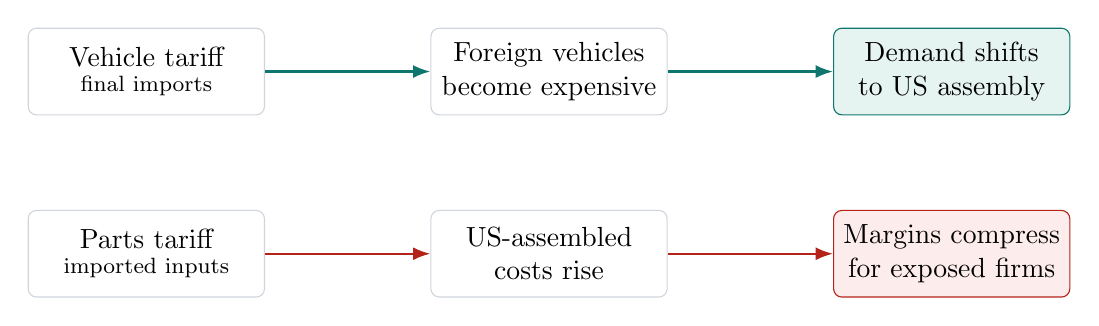
\begin{tikzpicture}[
    node distance=1.0cm,
    box/.style={draw=linegray, rounded corners=3pt, fill=white, minimum height=1.1cm, minimum width=3.0cm, align=center},
    arrow/.style={-{Latex[length=2.2mm]}, thick}
  ]
    \node[box] (vehicle) {Vehicle tariff\\[-0.1cm]{\footnotesize final imports}};
    \node[box, right=2.1cm of vehicle] (foreign) {Foreign vehicles\\become expensive};
    \node[box, right=2.1cm of foreign, fill=tealLight, draw=teal] (gain) {Demand shifts\\to US assembly};

    \node[box, below=1.2cm of vehicle] (parts) {Parts tariff\\[-0.1cm]{\footnotesize imported inputs}};
    \node[box, right=2.1cm of parts] (domcost) {US-assembled\\costs rise};
    \node[box, right=2.1cm of domcost, fill=redLight, draw=red] (loss) {Margins compress\\for exposed firms};

    \draw[arrow, teal] (vehicle) -- (foreign);
    \draw[arrow, teal] (foreign) -- (gain);
    \draw[arrow, red] (parts) -- (domcost);
    \draw[arrow, red] (domcost) -- (loss);
  \end{tikzpicture}
  \end{center}
  \vspace{0.25cm}
  \begin{center}
    \textbf{We ask how accounting for tariffs on parts changes the results of automotive tariffs.}
  \end{center}
\end{frame}

% 5
\begin{frame}{Setting: new automotive tariffs target vehicles and components}
  \textbf{Actual tariff regime}
  \begin{itemize}
    \item Section 232 auto package: 25\% additional tariffs on imported vehicles and automotive components.
    \item Tariff rates are lower for the UK (10\%), Japan (15\%), and South Korea (15\%).
  \end{itemize}
\end{frame}

% 6
\begin{frame}{Setting: US automotive market is highly exposed to imports}
  \begin{columns}[T,onlytextwidth]
    \column{0.43\textwidth}
      \begin{itemize}
        \item In the 2024 counterfactual market, 53.2\% of US light-duty vehicle sales are assembled in the United States.
        \item Among US-assembled vehicles, 54.1\% of parts value is foreign, sales-weighted.
        \item The included figure shows heterogeneity in foreign-parts reliance across domestically assembled vehicle lines.
      \end{itemize}
    \column{0.53\textwidth}
      \includegraphics[width=\linewidth]{\asset{domestic_share.png}}
      \srcnote{Figure reports US/Canada parts share by value. Foreign share is one minus that measure.}
  \end{columns}
\end{frame}

% 6
\begin{frame}{Results preview: parts tariffs reverse producer gains; EV subsidies boost consumer surplus}
  \centering
  \renewcommand{\arraystretch}{1.20}
  \begin{tabular}{lccc}
    \toprule
    & Vehicle tariff & Vehicle + parts tariff & EV subsidy \\
    & C1 & C2 & C3 \\
    \midrule
    Average price & \(+5.67\%\) & \(+9.36\%\) & \(-0.06\%\) \\
    Consumer surplus & \(-\$15.1b\) & \(-\$31.0b\) & \(+\$10.1b\) \\
    US producer surplus & \textcolor{teal}{\(+\$1.04b\)} & \textcolor{red}{\(-\$2.09b\)} & \textcolor{teal}{\(+\$1.80b\)} \\
    US assembled output & \(+1.25m\) & \(+0.12m\) & \(+0.14m\) \\
    EV share of sales & \(3.18\%\) & \(3.16\%\) & \textcolor{teal}{\(7.39\%\)} \\
    \bottomrule
  \end{tabular}
\end{frame}

% 7
\begin{frame}{Roadmap: how we model the impacts of tariffs}
  \begin{enumerate}
    \item Build a demand system to understand how consumers substitute between products when prices change.
    \item Use this demand system to recover marginal costs of each product.
    \item Estimate how changes in the price of foreign parts affects the cost of domestically produced vehicles.
  \end{enumerate}
  \vspace{0.45cm}
  \begin{center}
  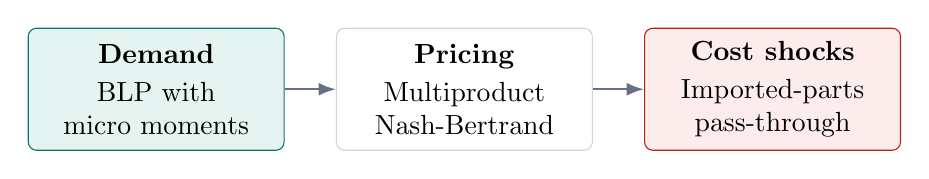
\begin{tikzpicture}[
    node distance=0.8cm,
    box/.style={draw=linegray, rounded corners=3pt, fill=white, minimum height=1.55cm, minimum width=3.25cm, align=center},
    arrow/.style={-{Latex[length=2.2mm]}, thick, draw=muted}
  ]
    \node[box, fill=tealLight, draw=teal] (demand) {\textbf{Demand}\\[0.06cm]BLP with\\micro moments};
    \node[box, right=0.65cm of demand] (supply) {\textbf{Pricing}\\[0.06cm]Multiproduct\\Nash-Bertrand};
    \node[box, right=0.65cm of supply, fill=redLight, draw=red] (costs) {\textbf{Cost shocks}\\[0.06cm]Imported-parts\\pass-through};
    \draw[arrow] (demand) -- (supply);
    \draw[arrow] (supply) -- (costs);
  \end{tikzpicture}
  \end{center}
\end{frame}

\begin{frame}{Data inputs}
  \begin{itemize}
    \item \textbf{Sales data}
      \begin{itemize}
        \item S\&P Polk registration microdata; ZIP-by-trim registrations converted to new-sales proxies and aggregated to model-year products.
      \end{itemize}
    \item \textbf{Characteristics data}
      \begin{itemize}
        \item DataOne trim-level vehicle characteristics; median price, size, horsepower, weight, fuel economy, powertrain, and assembly location.
      \end{itemize}
    \item \textbf{Imported parts by product}
      \begin{itemize}
        \item NHTSA/AALA manufacturing reports: assembly location, US/Canada parts share, and country-of-origin shares for foreign countries above 15\% of parts value.
      \end{itemize}
    \item \textbf{Consumer data}
      \begin{itemize}
        \item IPUMS household demographics by location and income; CEX new-vehicle expenditure moments for income-based purchase patterns.
      \end{itemize}
  \end{itemize}
  \vfill
  \begin{center}
    \textcolor{teal}{\bfseries Vehicle panel covers 2015--2024.}
  \end{center}
\end{frame}

\begin{frame}[plain]
  \vspace{1.0cm}
  {\Huge\bfseries Model}
\end{frame}

\begin{frame}{Why use a BLP demand system?}
  \begin{itemize}
    \item Tariffs move relative prices across hundreds of differentiated vehicle models; incidence depends on where consumers substitute.
    \item Random coefficients allow price sensitivity and tastes for size, performance, and powertrain to vary across consumers.
    \item The implied demand derivatives feed the supply side, recovering product-level marginal costs and markups under multiproduct Nash-Bertrand pricing.
    \item Micro moments discipline the key objects: demographic purchase patterns and first--second choice correlations pin down heterogeneity and substitution.
  \end{itemize}
\end{frame}

% 9
\begin{frame}{Demand identifies the substitution patterns behind incidence}
  \begin{columns}[T,onlytextwidth]
    \column{0.55\textwidth}
      \[
      u_{ijt}=\phi_{it}+\beta_i'X_{jt}+\alpha_{it}(p_{jt}-\tau_{jt})+\xi_{jt}+\varepsilon_{ijt}
      \]
      \begin{itemize}
        \item Consumers choose among vehicles and the outside option.
        \item Price enters net of EV subsidy.
        \item Income and region shift tastes and price sensitivity.
      \end{itemize}
    \column{0.36\textwidth}
      \textbf{Characteristics considered}
      \begin{itemize}
        \item Price, subsidy, size, horsepower, fuel economy.
        \item EV, hybrid, van, truck, SUV.
        \item Euro brand, luxury brand, firm effects, year effects.
        \item Income and Census-division interactions.
      \end{itemize}
  \end{columns}
\end{frame}

\begin{frame}{Nonlinear demand estimates imply rich substitution patterns}
  \scriptsize
  \begin{columns}[T,onlytextwidth]
    \column{0.48\textwidth}
      \textbf{Random coefficient standard deviations, \(\sigma\)}
      \vspace{0.1cm}
      \begin{tabular}{lr}
        \toprule
        Characteristic & Coef (s.e.) \\
        \midrule
        \(\log(\text{mpg}_{ICE/Hyb})\) & 5.753 (1.049) \\
        \(\log(\text{hp})\) & 1.957 (0.184) \\
        Van & 6.581 (1.672) \\
        Truck & 12.456 (3.192) \\
        SUV & 2.640 (0.323) \\
        EV & 1.996 (0.987) \\
        Euro brand & 2.074 (0.392) \\
        Luxury brand & 2.707 (0.468) \\
        \bottomrule
      \end{tabular}
    \column{0.50\textwidth}
      \textbf{Demographic and regional heterogeneity, \(\pi\)}
      \vspace{0.1cm}
      \begin{tabular}{lr}
        \toprule
        Interaction & Coef (s.e.) \\
        \midrule
        Intercept \(\times \log(\text{income}_{10k})\) & 3.935 (0.931) \\
        Price net subsidy \(\times \log(\text{income}_{10k})\) & 4.679 (1.563) \\
        Truck \(\times\) North Central & 3.512 (2.051) \\
        Truck \(\times\) South Central & 3.229 (2.103) \\
        Truck \(\times\) Mountain & 3.595 (2.806) \\
        SUV \(\times\) North East & 0.625 (0.531) \\
        SUV \(\times\) North Central & 0.553 (0.505) \\
        EV \(\times\) North East & 0.893 (1.056) \\
        EV \(\times\) South Atlantic & 0.693 (1.113) \\
        EV \(\times\) Mountain & 1.290 (1.383) \\
        EV \(\times\) Pacific & 3.204 (1.059) \\
        \bottomrule
      \end{tabular}
  \end{columns}
  \srcnote{Standard errors clustered by model.}
\end{frame}

% 10
\begin{frame}{Micro moments provide information on consumer substitution patterns and demographic differences}
  \begin{columns}[T,onlytextwidth]
    \column{0.39\textwidth}
      \begin{itemize}
        \item Income moments: purchase probabilities and expected prices by income quintile.
        \item Geography moments: EV, truck, and SUV shares by division.
        \item Second-choice moments: published substitution evidence for 2015 and 2022.
      \end{itemize}
    \column{0.61\textwidth}
      \scriptsize
      \begin{tabular}{@{}lrrr@{}}
        \toprule
        Moment & Data & Model & Diff. \\
        \midrule
        Price Q5--Q1 & 0.063 & 0.071 & -0.008 \\
        Purchase Q5/Q1 & 5.841 & 5.448 & +0.393 \\
        2nd truck \(|\) 1st truck & 0.872 & 0.889 & -0.017 \\
        2nd EV \(|\) 1st EV & 0.520 & 0.500 & +0.020 \\
        Pacific EV share, 2021 & 0.083 & 0.102 & -0.019 \\
        S. Central truck share, 2021 & 0.212 & 0.236 & -0.024 \\
        \bottomrule
      \end{tabular}
  \end{columns}
\end{frame}

% 11
\begin{frame}{Example diversion ratios show within-segment substitution}
  \scriptsize
  \renewcommand{\arraystretch}{1.18}
  \begin{tabularx}{\textwidth}{@{}>{\bfseries}p{0.23\textwidth}>{\raggedright\arraybackslash}X@{}}
    \toprule
    Product & Top destinations if buyers leave the product \\
    \midrule
    Tesla Model 3 EV & Outside good 38.2\%; Tesla Model Y EV 14.6\%; BMW i4 EV 2.4\% \\
    Toyota RAV4 Hybrid & Outside good 30.1\%; Honda CR-V Hybrid 9.3\%; Hyundai Tucson Hybrid 4.1\% \\
    Ford Bronco & Outside good 18.0\%; Jeep Grand Cherokee 3.9\%; Chevrolet Tahoe 3.0\% \\
    Audi A5 & Outside good 12.1\%; Mercedes-Benz C-Class 4.9\%; BMW 3 Series 2.7\% \\
    Honda Civic & Outside good 10.3\%; Toyota Corolla 5.8\%; Nissan Rogue 4.9\% \\
    Ford F-150 & Chevrolet Silverado 29.2\%; GMC Sierra 15.6\%; Outside good 6.8\% \\
    \bottomrule
  \end{tabularx}
  \vspace{0.35cm}
  \begin{itemize}
    \item Diversion ratios are the share of consumers switching away from a product who substitute toward each alternative.
    \item This is the demand-side object that governs where tariff-induced price changes redirect sales.
  \end{itemize}
\end{frame}

% 12
\begin{frame}{Supply recovers marginal costs from multiproduct pricing}
  \begin{center}
    \includegraphics[width=0.84\linewidth]{\asset{markups_dist.png}}
  \end{center}
  \vspace{-0.15cm}
  \small
  \begin{itemize}
    \item Share-weighted average markup across the full sample: \textbf{17.2\%}.
    \item Share-weighted mean own-price elasticity: \textbf{\(-6.764\)}.
  \end{itemize}
\end{frame}

% 12
\begin{frame}{We estimate the effect of foreign-parts price changes on vehicle marginal costs}
  \[
  \log(mc_{jt})=
  \gamma'\log(X_{jt})
  +\eta\left(\rho^{(1)}_{f,j,t-1}\log(RER^{(1)}_{jt})\right)
  +\lambda_j+\lambda_t+\epsilon_{jt}
  \]
  \vspace{0.15cm}
  \begin{itemize}
    \item \(\rho^{(1)}_{f,j,t-1}\): lagged exposure to the primary foreign parts country.
    \item \(RER^{(1)}_{jt}\): bilateral real exchange-rate shock for that country.
    \item Lagged exposure addresses endogeneity concerns: contemporaneous \(RER\) shocks can mechanically change reported foreign-parts value and may induce firms to reduce imported-parts shares.
    \item Preferred estimate: \(\eta=0.602\), meaning incomplete cost transmission.
  \end{itemize}
\end{frame}

\begin{frame}{Estimated cost-side coefficients}
  \centering
  \small
  \renewcommand{\arraystretch}{1.15}
  \begin{tabular}{lcc}
    \toprule
    & Levels + controls & First differences + controls \\
    \midrule
    \(\log(\text{size})\) & 0.548 (0.201) & 0.541 (0.254) \\
    \(\log(\text{weight})\) & 0.300 (0.176) & 0.407 (0.223) \\
    \(\log(\text{hp})\) & 0.206 (0.081) & 0.251 (0.098) \\
    \(\log(\text{mpg})\) & -0.087 (0.074) & -0.046 (0.070) \\
    \(\rho^{(1)}_{f,j,t-1}\times \log(RER^{(1)}_{jt})\) & \textbf{0.602 (0.229)} & 0.513 (0.214) \\
    \midrule
    Observations & 384 & 262 \\
    \(R^2\) & 0.979 & 0.178 \\
    \bottomrule
  \end{tabular}
  \vspace{0.25cm}
  \par{\scriptsize\textcolor{muted}{Dependent variable is \(\log(\text{marginal cost})\). Standard errors clustered by make-model.}}
\end{frame}

% 13
\begin{frame}{Counterfactuals re-solve prices in the 2024 market}
  \begin{columns}[T,onlytextwidth]
    \column{0.49\textwidth}
      \textbf{Vehicle tariff channel}
      \[
      mc^{(f)}_{CF}=mc^{(f)}_{0}(1+\tau \cdot tariff_{j})
      \]
      \begin{itemize}
        \item Imported final vehicles receive country-specific tariff rates.
      \end{itemize}
    \column{0.49\textwidth}
      \textbf{Parts tariff channel}
      \[
      mc^{(d)}_{CF}=mc^{(d)}_{0}(1+\eta\rho_f \cdot tariff_{parts})
      \]
      \begin{itemize}
        \item US-assembled cost shock scales with imported-parts exposure.
      \end{itemize}
  \end{columns}
  \vfill
  \srcnote{Product offerings and assembly locations are fixed; firms re-optimize prices.}
\end{frame}

\begin{frame}[plain]
  \vspace{1.0cm}
  {\Huge\bfseries Results}
\end{frame}

% 15
\begin{frame}{Vehicle-only tariffs look like standard protection}
  \begin{columns}[T,onlytextwidth]
    \column{0.42\textwidth}
      \textbf{C1: tariff imported vehicles only}
      \begin{itemize}
        \item Foreign-assembled marginal costs rise sharply.
        \item Domestic prices barely move.
        \item US-assembled market share increases by 5.66 pp.
      \end{itemize}
      \vspace{0.25cm}
      \textcolor{teal}{\bfseries US producer surplus rises by \$1.04b.}
      \vspace{0.15cm}

      \textcolor{red}{\bfseries Consumer surplus falls by \$15.1b.}
    \column{0.54\textwidth}
      \includegraphics[width=\linewidth]{\asset{origin_metrics_vehicles_only_tariff__no_subsidy.png}}
  \end{columns}
\end{frame}

% 16
\begin{frame}{Adding parts tariffs turns protection into a broad cost shock}
  \begin{columns}[T,onlytextwidth]
    \column{0.42\textwidth}
      \textbf{C2: tariff vehicles and parts}
      \begin{itemize}
        \item US-assembled marginal costs rise 8.15\%.
        \item US-assembled prices rise 7.08\%.
        \item Domestic share gains are much smaller.
      \end{itemize}
      \vspace{0.25cm}
      \textcolor{red}{\bfseries US producer surplus falls by \$2.09b.}
      \vspace{0.15cm}

      \textcolor{red}{\bfseries Consumer surplus falls by \$31.0b.}
    \column{0.54\textwidth}
      \includegraphics[width=\linewidth]{\asset{origin_metrics_parts_and_vehicles_tariff__no_subsidy.png}}
  \end{columns}
\end{frame}

\begin{frame}{EV subsidy reenactment expands the market and EV adoption}
  \begin{columns}[T,onlytextwidth]
    \column{0.43\textwidth}
      \textbf{C3: no tariff, EV subsidy}
      \begin{itemize}
        \item Average prices barely move because the subsidy applies to a subset of products.
        \item Consumer surplus rises by \(\$10.1b\).
        \item EV share of vehicles sold rises from \(3.36\%\) to \(7.39\%\).
      \end{itemize}
    \column{0.53\textwidth}
      \centering
      \renewcommand{\arraystretch}{1.18}
      \small
      \begin{tabular}{lc}
        \toprule
        & C3: EV subsidy \\
        \midrule
        Average price & \(-0.06\%\) \\
        Consumer surplus & \(+\$10.1b\) \\
        US producer surplus & \(+\$1.80b\) \\
        Vehicles sold & \(+0.20m\) \\
        EV sales & \(840k\) \\
        EV share of sales & \(7.39\%\) \\
        US assembled output & \(+0.14m\) \\
        EV subsidy cost & \(\$6.68b\) \\
        \bottomrule
      \end{tabular}
  \end{columns}
\end{frame}

\begin{frame}{EV sales rise sharply when subsidies return}
  \begin{center}
    \includegraphics[width=\linewidth,height=0.78\textheight,keepaspectratio]{\asset{ev_share_sales_by_scenario_compact.png}}
  \end{center}
\end{frame}

% 17
\begin{frame}{Scenario comparison}
  \centering
  \small
  \renewcommand{\arraystretch}{1.15}
  \begin{tabular}{lccc}
    \toprule
    & C1: vehicles only & C2: vehicles + parts & C3: EV subsidy \\
    \midrule
    Average price & \(+5.67\%\) & \(+9.36\%\) & \(-0.06\%\) \\
    Consumer surplus & \(-\$15.1b\) & \(-\$31.0b\) & \textcolor{teal}{\(+\$10.1b\)} \\
    US producer surplus & \textcolor{teal}{\(+\$1.04b\)} & \textcolor{red}{\(-\$2.09b\)} & \textcolor{teal}{\(+\$1.80b\)} \\
    Vehicles sold & \(-0.41m\) & \(-0.83m\) & \(+0.20m\) \\
    EV share (\% sales) & \(3.18\%\) & \(3.16\%\) & \textcolor{teal}{\(7.39\%\)} \\
    US assembled (\# vehicles) & \(+1.25m\) & \(+0.12m\) & \(+0.14m\) \\
    Tariff revenue & \(+\$15.38b\) & \(+\$41.55b\) & \(\$0.00b\) \\
    EV subsidy cost & \(\$0.00b\) & \(\$0.00b\) & \(\$6.68b\) \\
    \bottomrule
  \end{tabular}
\end{frame}

\begin{frame}{Consumer surplus impacts vary by income quintile}
  \vspace{-0.15cm}
  \begin{center}
    \includegraphics[width=\linewidth,height=0.80\textheight,keepaspectratio]{\asset{cs_quintile_grouped_bars.png}}
  \end{center}
\end{frame}

\begin{frame}{Firm outcomes depend on input exposure, not headquarters alone}
  \vspace{-0.1cm}
  \begin{center}
    \includegraphics[width=\linewidth,height=0.82\textheight,keepaspectratio]{\asset{z_scatter_pct_more.png}}
  \end{center}
\end{frame}

\begin{frame}{Firm-level profit changes: C1 vehicle-only tariff}
  \begin{center}
    \includegraphics[width=\linewidth,height=0.75\textheight,keepaspectratio]{\asset{profit_changes_vehicles_only_tariff__no_subsidy.png}}
  \end{center}
  \vspace{-0.2cm}
  \srcnote{Bars report profit changes relative to B0. Blue bars are US-headquartered firms.}
\end{frame}

\begin{frame}{Firm-level profit changes: C2 vehicle + parts tariffs}
  \begin{center}
    \includegraphics[width=\linewidth,height=0.75\textheight,keepaspectratio]{\asset{profit_changes_parts_and_vehicles_tariff__no_subsidy.png}}
  \end{center}
  \vspace{-0.2cm}
  \srcnote{Bars report profit changes relative to B0. Blue bars are US-headquartered firms.}
\end{frame}

\begin{frame}{Firm-level profit changes: C3 EV subsidy}
  \begin{center}
    \includegraphics[width=\linewidth,height=0.75\textheight,keepaspectratio]{\asset{profit_changes_no_tariff__with_subsidy.png}}
  \end{center}
  \vspace{-0.2cm}
  \srcnote{Bars report profit changes relative to B0. Blue bars are US-headquartered firms.}
\end{frame}

\begin{frame}{EV sales changes concentrate among major EV producers}
  \vspace{-0.12cm}
  \begin{center}
    \includegraphics[width=\linewidth,height=0.78\textheight,keepaspectratio]{\asset{ev_firm_sales_change_c1_c3.png}}
  \end{center}
  \vspace{-0.30cm}
  \srcnote{Changes are relative to B0. Firms are grouped by owner.}
\end{frame}

% 20
\begin{frame}{Tariff regime choice affects production locations}
  \begin{columns}[T,onlytextwidth]
    \column{0.49\textwidth}
      \includegraphics[width=\linewidth]{\asset{assembly_map_vehicles_only_tariff__no_subsidy.png}}
    \column{0.49\textwidth}
      \includegraphics[width=\linewidth]{\asset{assembly_map_parts_and_vehicles_tariff__no_subsidy.png}}
  \end{columns}
  \srcnote{Left: vehicle-only tariff. Right: vehicle and parts tariffs. Both are relative to no tariff, no subsidy.}
\end{frame}

\begin{frame}{What to take away}
  \begin{enumerate}
    \item \textbf{Final-goods protection can help domestic producers.}\\
    In this market, a vehicle-only tariff raises US producer surplus by about \(\$1b\).
    \vspace{0.18cm}
    \item \textbf{Input tariffs can reverse that gain.}\\
    Adding parts tariffs roughly doubles consumer losses and lowers US producer surplus by about \(\$2.1b\).
    \vspace{0.18cm}
    \item \textbf{EV subsidy reenactment greatly expands consumer surplus and EV share.}\\
    It raises consumer surplus by \(\$10.1b\) and increases EV share of sales from \(3.36\%\) to \(7.39\%\).
  \end{enumerate}
\end{frame}

\sectionframe{Backup}{Additional tables and robustness}

% B1
\begin{frame}{Backup: regional consumer gains follow EV preferences and incomes}
  \begin{columns}[T,onlytextwidth]
    \column{0.38\textwidth}
      \begin{itemize}
        \item Welfare gains are broad across states.
        \item Gains are larger in high-EV-preference regions.
        \item Oregon, Washington, California, Alaska, and Hawaii stand out.
      \end{itemize}
    \column{0.58\textwidth}
      \includegraphics[width=\linewidth]{\asset{cs_map_no_tariff__with_subsidy.png}}
  \end{columns}
\end{frame}

% B2
\begin{frame}{Backup: what the analysis abstracts from}
  \begin{itemize}
    \item Product offerings and assembly locations are fixed in the 2024 counterfactuals.
    \item Long-run entry, exit, plant relocation, and deep supplier-network redesign are outside the model.
    \item AALA data report US and Canadian parts together, so Canadian input exposure is not separately identified.
    \item Sourcing choices enter through the estimated pass-through sufficient statistic rather than a structural supplier-choice model.
  \end{itemize}
  \vfill
  \begin{center}
    \textbf{These limits make the estimates medium-run incidence results, not long-run industrial-policy forecasts.}
  \end{center}
\end{frame}

% B3
\begin{frame}{Backup: full six-scenario counterfactual summary}
  \centering
  \scriptsize
  \renewcommand{\arraystretch}{1.16}
  \begin{tabular}{lrrrrrr}
    \toprule
    & B0 & C1 & C2 & C3 & C4 & C5 \\
    \midrule
    Price \(\Delta\) (\%) & 0.00 & 5.67 & 9.36 & -0.06 & 5.61 & 9.30 \\
    US PS \(\Delta\) (\$b) & 0.00 & 1.04 & -2.09 & 1.80 & 3.12 & -0.10 \\
    CS \(\Delta\) (\$b) & 0.00 & -15.09 & -31.04 & 10.06 & -6.19 & -22.66 \\
    Vehicles sold \(\Delta\) (m) & 0.00 & -0.41 & -0.83 & 0.20 & -0.22 & -0.65 \\
    EV share (\% sales) & 3.36 & 3.18 & 3.16 & 7.39 & 6.75 & 6.67 \\
    Tariff revenue (\$b) & 0.00 & 15.38 & 41.55 & 0.00 & 15.67 & 42.21 \\
    Subsidy cost (\$b) & 0.00 & 0.00 & 0.00 & 6.68 & 6.00 & 5.63 \\
    Net US impact (\$b) & 0.00 & 1.33 & 8.43 & 5.17 & 6.60 & 13.83 \\
    \bottomrule
  \end{tabular}
  \vspace{0.35cm}
  \srcnote{C1/C2 are without subsidy; C3/C4/C5 are with subsidy. C4 is vehicle-only tariff with subsidy; C5 is vehicle+parts tariff with subsidy.}
\end{frame}

% B4
\begin{frame}{Backup: distribution of consumer price sensitivity}
  \begin{columns}[T,onlytextwidth]
    \column{0.42\textwidth}
      \begin{itemize}
        \item Estimated price disutility varies with income.
        \item This heterogeneity drives distributional CS results.
        \item Higher-income buyers account for more vehicle purchases.
      \end{itemize}
    \column{0.55\textwidth}
      \includegraphics[width=\linewidth]{\asset{price_coef.png}}
  \end{columns}
\end{frame}

\end{document}
